\section{Banco de dados}

Feita a analise das relações geométricas entre as estrelas presentes no FOV, com as informações, de momentos, áreas e momentos angulares, 
é então inicializado a pesquisa no banco de dados interno do cubesat, para verificarão de possíveis estrelas.

Devido às limitações energéticas do sistema, é necessário que a estrutura do banco de dados seja otimizada para a resolução do problema em questão.
Além disto o próprio processo de geração do banco de dados que também requer uma otimização, para que o mesmo seja gerado em um tempo aceitável.
Pois, a combinação de 3 estrelas diferentes para realização do calculo da area e do momento pode gerar um problema de O(n\textsuperscript{3}).

Além disto a técnicas de busca e analise de resultados também devem ser otimizadas e levar levar em consideração múltiplos fatores.
Cabe ressaltar que a operação do sistema de orientação e controle do cubesat possui duas fases distintas de operação, a fase em que não há informação previa de localização e a fase em que já há informação previa de localização.
Neste trabalho é apenas abordada a fase em que não há informação previa de localização.

\subsection{Gerando o banco de dados}
Após a análise de imagem o sistema precisa compar os resultados das leituras com um banco de dados de estrelas, para que seja possível identificar a posição do cubesat, 
relacionando a posição da estrela observada a posição do cubesat, 
o banco de dados é composto por algumas partes, sendo elas:
\begin{itemize}
    \item \textbf{Relações Áreas e Momentos angulares}: Lista ordenada da combinação de 3 estrelas. Contendo as informações de área e momento angular, juntamente com o identificador das estrelas Figura \ref{fig:banco_dados_area_moment_to_cubesat}.
    \item \textbf{Relações de Ângulos entre estrelas}: Lista ordenada da combinação de 2 estrelas. Contendo as informações de ângulo entre as estrelas, juntamente com o identificador das estrelas Figura \ref{fig:banco_dados_angulo}.
    \item \textbf{Relação de id e posição estrelar}: Este é o mesmo banco de dados utilizado para gerar a simulação, contendo as informações de id e posição estrelar Figura \ref{fig:banco_dados_posicao}.
\end{itemize}

\begin{figure}[H]
    \centering
    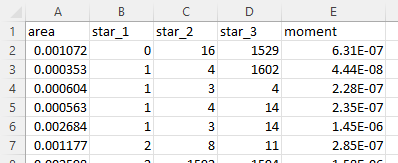
\includegraphics[width=0.7\textwidth]{images/banco_dados_area_moment.png}
    \caption{Parte do arquivo de banco de dados de áreas e momentos angulares, Fonte: Autoria própria}
    \label{fig:banco_dados_area_moment_to_cubesat}
\end{figure}

\begin{figure}[H]
    \centering
    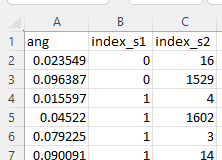
\includegraphics[width=0.35\textwidth]{images/banco_dados_angulo.png}
    \caption{Parte do arquivo de banco de dados de ângulos entre estrelas, Fonte: Autoria própria}
    \label{fig:banco_dados_angulo}
\end{figure}

\begin{figure}[H]
    \centering
    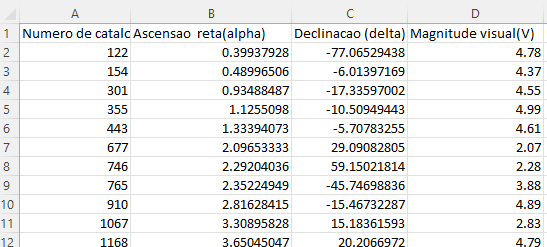
\includegraphics[width=0.7\textwidth]{images/banco_dados_posicao.png}
    \caption{Parte do arquivo de banco de dados de posição estrelar, Fonte: Autoria própria}
    \label{fig:banco_dados_posicao}
\end{figure}

\subsubsection{Octree}

Nota-se que a combinação de 3 estrelas diferentes para realização do cálculo da área e do momento pode gerar um problema de complexabilidade O(n\textsuperscript{3}),
Porém, apenas estrelas próximas uma as outras que podem geram uma combinação de area valida para a analise.
Nota-se que apenas estrelas dentro de um circulo ao redor da estrela central podem gerar uma combinação de area valida para a analise, como visto na Figura \ref{fig:estrelas_endorno}.

\begin{figure}[H]
    \centering
    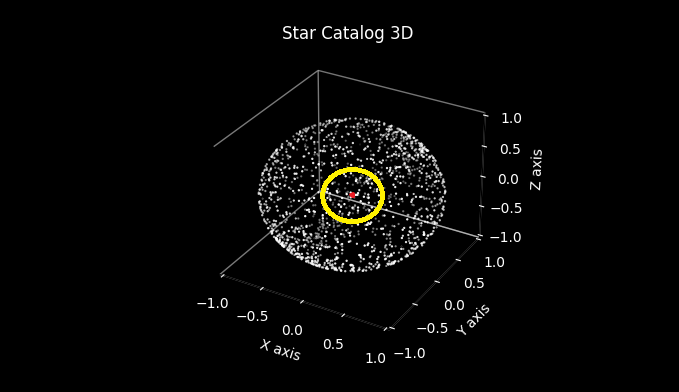
\includegraphics[width=0.8\textwidth]{images/estrelas_endorno.png}
    \caption{Exemplo de Octo Tree, Fonte: \cite{octo_tree}}
    \label{fig:estrelas_endorno}
\end{figure}

Para se localizar de forma eficiente as estrelas ao retor de um circulo no espaço tridimensional, é utilizado a estrutura de dados Octree,
que é uma estrutura de dados que divide o espaço em 8 subespaços, como visto na Figura \ref{fig:octo_tree}. 
Dessa forma, calcula-se apenas areas e ângulos entre estrelas que estão dentro do circulo ao redor da estrela central.

\begin{figure}[H]
    \centering
    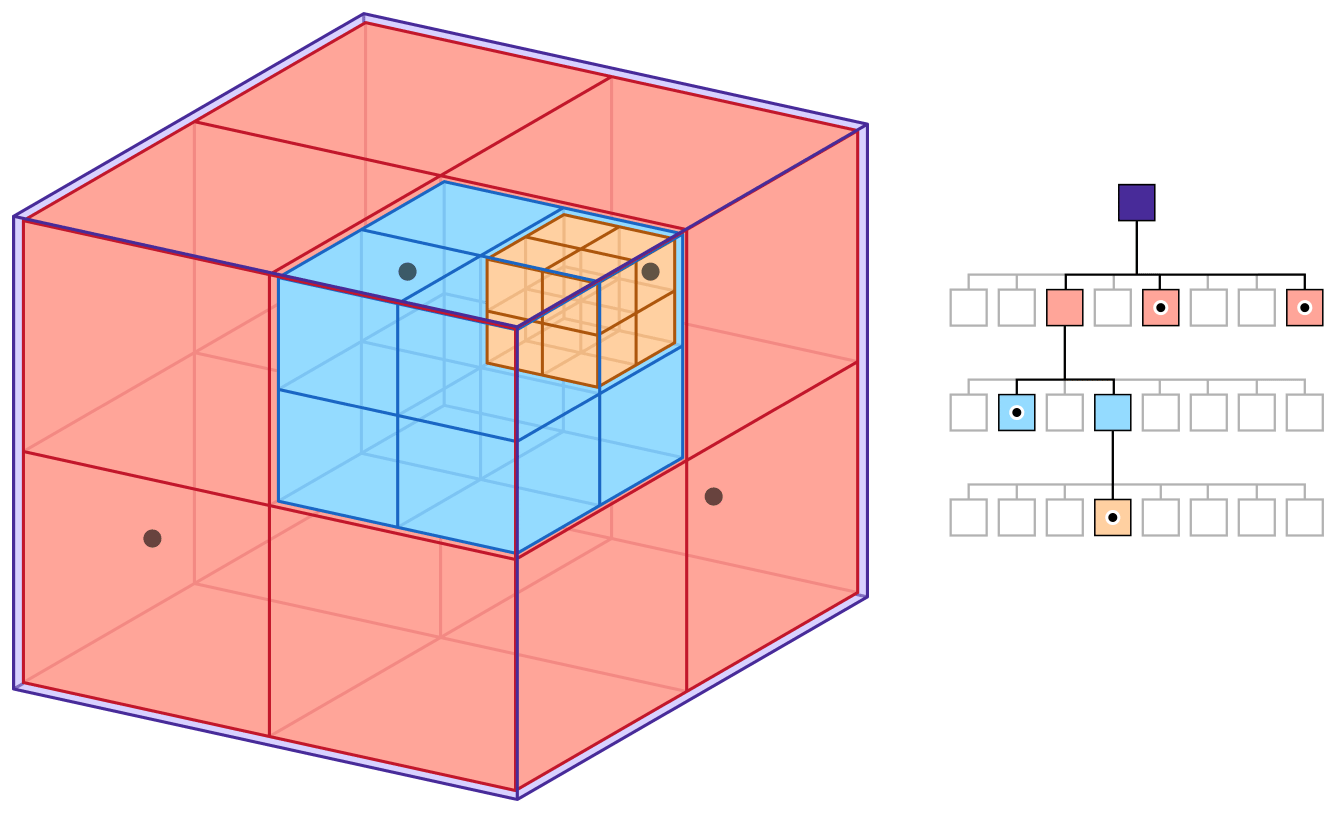
\includegraphics[width=0.8\textwidth]{images/octree.png}
    \caption{Exemplo de Octo Tree, Fonte: \cite{octo_tree}}
    \label{fig:octo_tree}
\end{figure}

\subsubsection{K vector}

O método \textbf{k vector} foi desenvolvido para refinar a faixa de busca em vetores ordenados de dados \cite{Mortari}.
Para que este método seja utilizado é necessário que todos os elementos do banco de dados sejam conhecidos previamente, 
pois o método consiste na criação de um modelo matemático relacionando a informação a ser encontrada, com o index do banco de dados.
Para isso,  a análise é inciada com a ordenação crescente dos dados. 
Apesar de não estritamente necessário, recomenda-se que seja plotado os em um  gráfico cartesiano, como na Figura ~\ref{fig:K_vector}.
Pois a elaboração de uma equação matemática que melhor represente a curva a ser encontrada, é mais fácil de ser feita com a visualização do gráfico.

A Figura ~\ref{fig:K_vector} mostra um exemplo de um gráfico de uma função linear, onde a equação matemática que melhor representa a curva é a equação da reta, 
porém isto não é uma regra, pois a curva pode ser uma função quadrática, cúbica, logarítmica, exponencial, etc.
\begin{figure}[h]
	\centering
	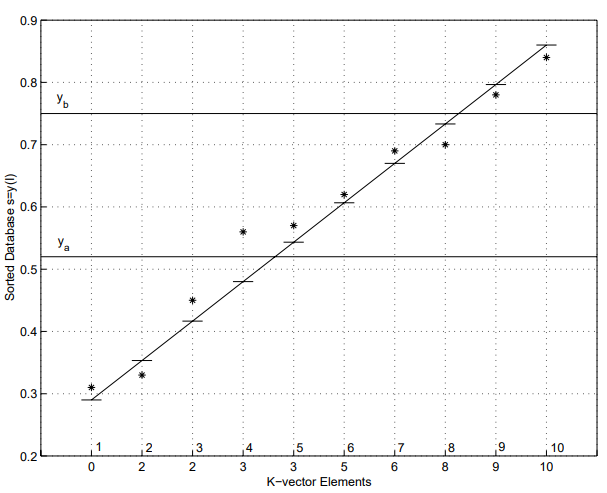
\includegraphics[width=0.5\textwidth]{images/k_vector.png}
	\caption{Exemplo da construção de um K vector. Fonte: ~\cite[]{Mortari}}
	\label{fig:K_vector} 
\end{figure}

No caso apresentado na Figura ~\ref{fig:K_vector}, pode-se utilizar, uma relação linear obtida através do método dos mínimos quadrados pelas equações ~\ref{eq:Beta_linear}, ~\ref{eq:Alpha_linear} e ~\ref{eq:Regressao_linear},

\begin{equation}
	\beta = \frac{\sum_{i=1}^{n} (x_i - \bar{x})(y_i - \bar{y})}{\sum_{i=1}^{n} (x_i - \bar{x})^2},
	\label{eq:Beta_linear}
\end{equation}

\begin{equation}
	\alpha = \bar{y} - \beta * \bar{x},
	\label{eq:Alpha_linear}
\end{equation}

\begin{equation}
	y = \alpha + \beta * x
	\label{eq:Regressao_linear}.
\end{equation}

Para explicar o funcionamento do método, será utilizado o exemplo da Figura ~\ref{fig:covid_1}.
Neste exemplo, objetivo é descobrir o dia em que um numero qualquer de novos casos de covid-19 ocorreram,
dessa forma se utiliza um método de regressão que melhor se encaixa na curva, em teremos como entrda \textbf{x} o numero de casos e como saída \textbf{y} o dia.

\begin{figure}[H]
    \centering
    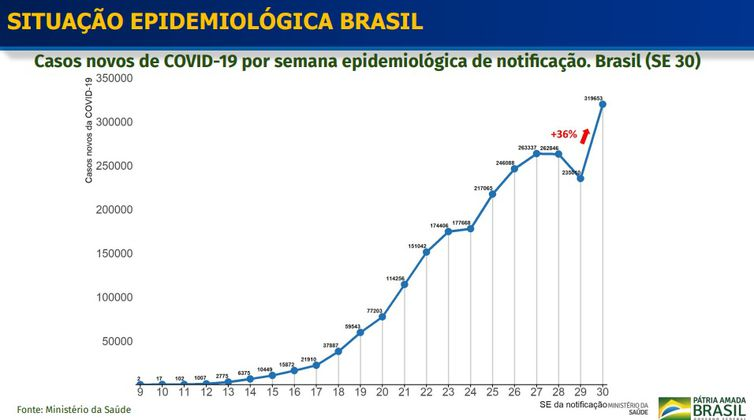
\includegraphics[width=0.5\textwidth]{images/covid_1.jpg}
    \caption{Casos Covid-19. Fonte: ~\cite[]{covid}}
    \label{fig:covid_1}
\end{figure}

Seja a curva vermelha presente na Figura ~\ref{fig:covid_2} a regressão que melhor satisfez aproximação da curva da Figura ~\ref{fig:covid_1}, 
está modelagem matemática apresenta de erros em sua aproximação, como pode se observar no desvio da curva vermelha em relação a curva azul.
Portando além do valor da regressão, é necessário calcular o erro da regressão ~\ref{fig:covid_3}, para que então possa se refinar a pesquisa em apenas uma parte dos set de dados.
Quando então algoritmo de busca binária é utilizado para finalizar a busca.
\begin{figure}[H]
    \centering
    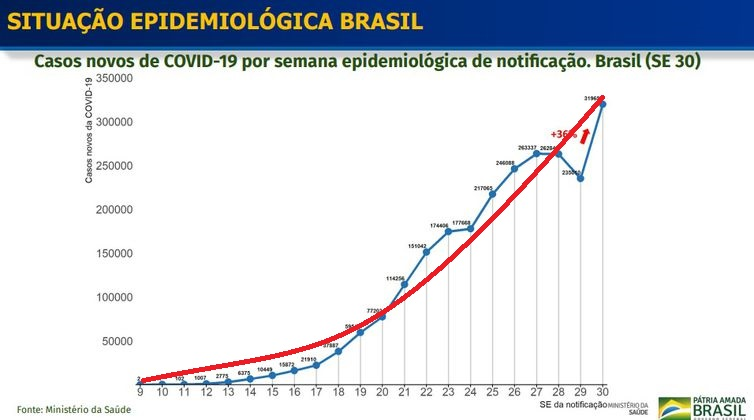
\includegraphics[width=0.5\textwidth]{images/covid_2.jpg}
    \caption{Curva de regressão, Fonte: Autoria Própria}
    \label{fig:covid_2}
\end{figure}

\begin{figure}[H]
    \centering
    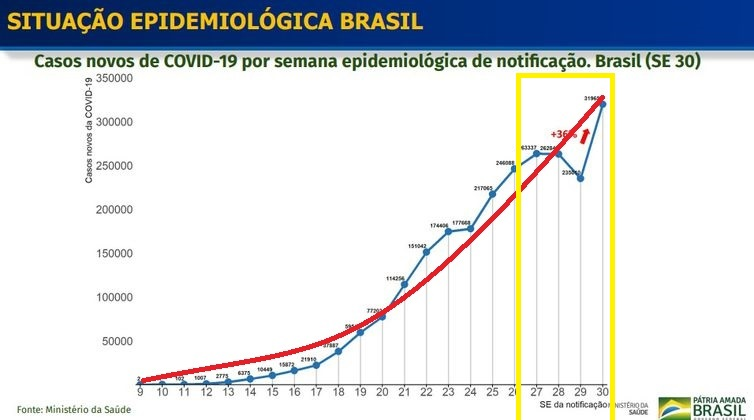
\includegraphics[width=0.5\textwidth]{images/covid_3.jpg}
    \caption{Possíveis dias para um certo numero de casos, Fonte: Autoria Própria}
    \label{fig:covid_3}
\end{figure}

Dessa forma o método consegue diminuir o tempo de pesquisa, ja que um vetor de tamanho \textbf{n}, com todas os valores conhecidos pode ter seu tempo busca reduzido do habitual O(n*log(n)) para O(2*error*log(2*error)), 
diminuí-se o tamanho do vetor de pesquisa a 2 vezes o erro máximo da linearização, dessa forma os algorítimos de busca binária só precisam executar a pesquisa neste vetor selecionado.
Neste trabalho, considero-se que o erro associado a aproximação é, o maior erro entre todos o valor calculado para todos o pontos da curva.

\subsection{Utilizando  o banco de dados}

Após o sistema de analise de imagem, medir os ângulos, areas e momentos triangulares entre as estrelas presentes na imagem, 
o sistema aplica um algótico de seleção de possibilidades, 
onde é selecionado as estrelas que possuem os ângulos e momentos triangulares mais próximos dos valores esperados.

\subsubsection{Pyramid}

Neste trabalho é utilizado o algorítimo de Pyramid, 
o algoritmo funciona da seguinte forma, 
primeiro é selecionado 3 estrelas, \textalpha, \textbeta  e \textgamma, 
com os valores de ângulos juntamente com o erro máximo da medição, é aplicado ao k-vector,
que gera 3 listas diferentes possibilidade.

Com estas listas filtradas é crias-se uma lista com todas as possíveis combinações de 3 estrelas, 
então é analisado o valor de area e momento triangular das estrelas no FOV, filtrado possíveis combinações que não se encaixam nos valores esperados.

Caso a analise resulte em mais de uma combinação possível, é realizado a analise de um segundo triangulo, 
o qual possui pelo menos uma estrela em comum com o primeiro triangulo, 
então o segundo triangulo é analisado da mesma forma que o primeiro.
Então os resultados dos dois triângulos são comparados, para selecionar apenas as possibilidades que estão presentes nos dois resultados.

Pode se visual o processo nas figuras ~\ref{fig:pyramid_1} e ~\ref{fig:pyramid_2} e ~\ref{fig:pyramid_3}.
\begin{figure}[H]
    \centering
    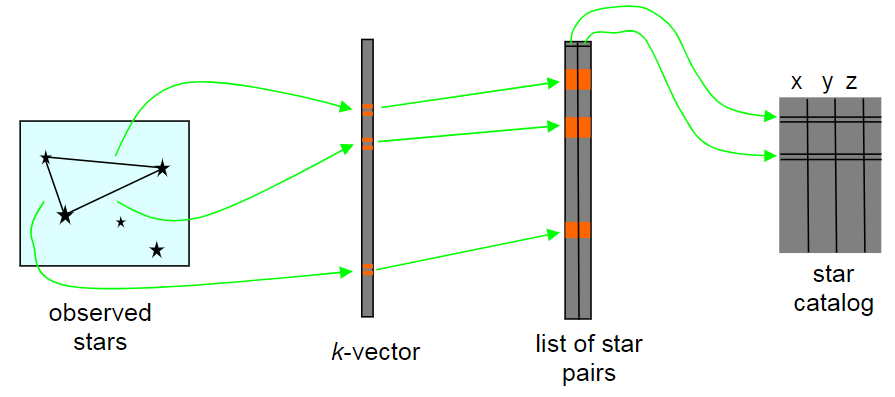
\includegraphics[width=1\textwidth]{images/Pyramid_01.png}
    \caption{Pyramid, Fonte: ~\cite[]{Fialho}}
    \label{fig:pyramid_01}
\end{figure}


\begin{figure}[H]
    \centering
    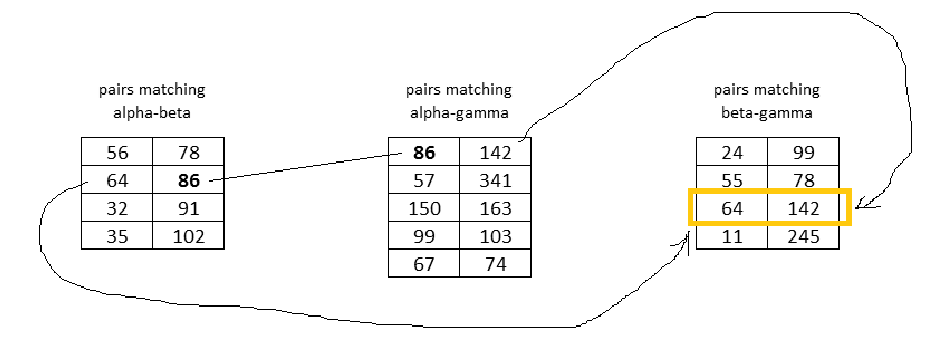
\includegraphics[width=1\textwidth]{images/Pyramid_02.png}
    \caption{Exemplo de Pyramid, Fonte: ~\cite[]{Fialho}}
    \label{fig:pyramid_02}
\end{figure}

\begin{figure}[H]
    \centering
    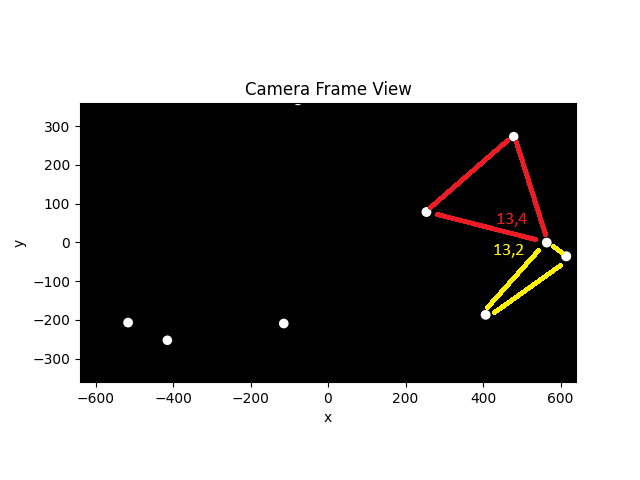
\includegraphics[width=1\textwidth]{images/Pyramid_03.png}
    \caption{Exemplo de Pyramid, Fonte: Autoria Própria}
    \label{fig:pyramid_03}
\end{figure}

No exemplo da Figura ~\ref{fig:pyramid_03}, a estrela que faz parte dos dois triângulos pode ser 13, 2 segundo a analise do triangulo amarelo, 
segundo a outra analise de pode-ser 13, 4 portando está estrela deve ser a 13.